\chapter{Технологическая часть}

В данном разделе будут приведены требования к программному обеспечению, средства реализации и листинги кода.


\section{Средства реализации}

В качестве языка программирования для реализации данной лабораторной работы был выбран язык программирования C\# \cite{sharplang}. 

Язык C\# является полностью объектно-ориентированным. 
Все необходимые библиотеки для реализации поставленной задачи являются стандартными.

Также в этом языке используются нативные потоки \cite{threads}.

Время работы алгоритмов было замерено с помощью класса Stopwatch \cite{cpplangtime}.

Для создания потоков использовалась библиотека System.Threading. 

\section{Сведения о модулях программы}
Программа состоит из следующих модулей.
\begin{enumerate}
	\item Programm.cs --- главный файл программы, в котором располагается код меню.
	\item Scene.cs --- файл с классом  сцены в котором располагаются методы исследуемых алгоритмов.
	\item Composite.cs, Cube.cs, LightSource.cs, LockBitmap.cs, Ray.cs, Trace.cs, SceneObject.cs, Sphere.cs, Trace.cs  --- файлы с кодами классов, необходимых для реализации обратной трассировки лучей.
\end{enumerate}


\section{Реализация алгоритмов}
В листингах \ref{lst:work}, \ref{lst:disp}, \ref{lst:fllw} представлены реализации алгоритмов, а именно алгоритм рабочего потока, потока диспетчера, и последовательного алгоритма обратной трассировки лучей.

\begin{lstlisting}[label=lst:work,caption=Метод рабочего потока]
private void RenderPiece(object parametrs)
{
	Params p = (Params)parametrs;
	int sw = p.WidthStart;
	int ew = p.WidthEnd;
	int sh = p.HeightStart;
	int eh = p.HeightEnd;

	for (int i = sw; i < ew; i++)
	for (int j = sh; j < eh; j++)
	{
		Trace t = TraceRay(i - (Cw / 2), -j + (Ch / 2));
		CastShadow(t);
		RenderSmoke(t);
		lbmp.SetPixel(i, j, t.Color);
	}
	sem[p.SemaphoreIndex] = false;
}
\end{lstlisting}

\begin{lstlisting}[label=lst:disp,caption=Метод потока диспетчера]
public void Render(int threadCount)
{
	Thread[] threads = new Thread[3 * (int)Math.Pow(2, threadCount + 1)];
	sem = new bool[3 * (int)Math.Pow(2, threadCount + 1)];
	int dtc = threadCount / 2;
	int mtc = threadCount % 2;
	int jh = 3 * (int)Math.Pow(2, dtc);
	int iw = (int)Math.Pow(2, dtc + mtc + 1);
	int k = 0;
	lbmp.LockBits();
	for (int i = 0; i < iw; i++)
	for (int j = 0; j < jh; j++)
	{
		sem[k] = true;
		
		threads[k] = new Thread(RenderPiece);
		threads[k].Start(new Params(i * Cw / iw, j * Ch / jh, (i + 1) * Cw / iw, (j + 1) * Ch / jh, k));
		k++;
	}
	bool f = true;
	while (f)
	{ 
		f = false;
		for (int i = 0; i < sem.Length; i++)
		if (sem[i])
		f = true;
	}
	lbmp.UnlockBits();
}
\end{lstlisting}

\begin{lstlisting}[label=lst:fllw,caption=Последовательный алгоритм обратной трассировки лучей]
public void RenderFollow()
{
	for (int i = 0; i < Cw; i++)
	for (int j = 0; j < Ch; j++)
	{
		Trace t = TraceRay(i - (Cw / 2), -j + (Ch / 2));
		CastShadow(t);
		RenderSmoke(t);
		bmp.SetPixel(i, j, t.Color);
	}
}
\end{lstlisting}

\section{Тестирование}

Тестирование выполнено по методологии белого ящика. Полученное изображение \ref{fig:test} совпадает с ожидаемым.
\begin{figure}[H]
	\centering
	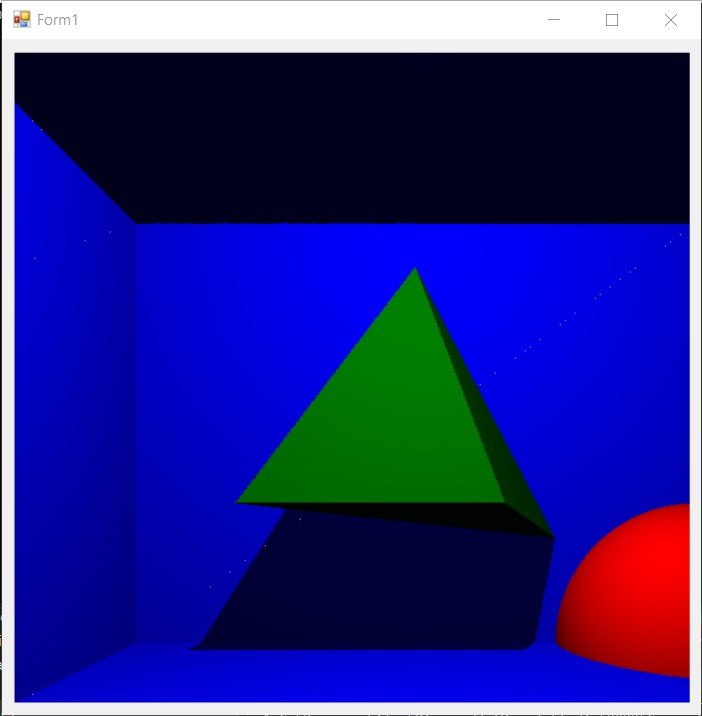
\includegraphics[width=1\linewidth]{inc/img/demographics}
	\caption{Полученное изображение в результате работы алгоритма}
	\label{fig:test}
\end{figure}
\section*{Вывод}

Были реализованы алгоритмы, а именно алгоритм рабочего потока, потока диспетчера, и последовательного алгоритма обратной трассировки лучей.
